\section{Grafy}
\label{sec:graphs}

Následují grafy pro dvanáct náhodně vybraných simulací pro uvedenou kombinaci parametrů.
Vždy znázorňují vývoj některé veličiny pro tyto simulace. Pro každou simulaci je veličina
vynášena jinou barvou do téhož grafu.

Tyto grafy si kladou za cíl pomoci snáze nahlédnout chování modelu v čase. K posouzení rozdílů mezi
různými nastaveními parametrů příliš vhodné nejsou, protože jde jen o velmi omezené počty simulací.


\subsection{Průměrná fitness}

Průměrná fitness roste díky selekci ve všech obdobích, přestože ne vždy stejným tempem. Mnoho populací končí vyhynutím.

\begin{figure}[H]
\caption{Graf vývojů průměrně fitness dvanácti populací pro podíl vznikajících pleiotropních alel 0.0 a pro podíl
         vznikajících negativně dominantních alel 0.0}
\centering
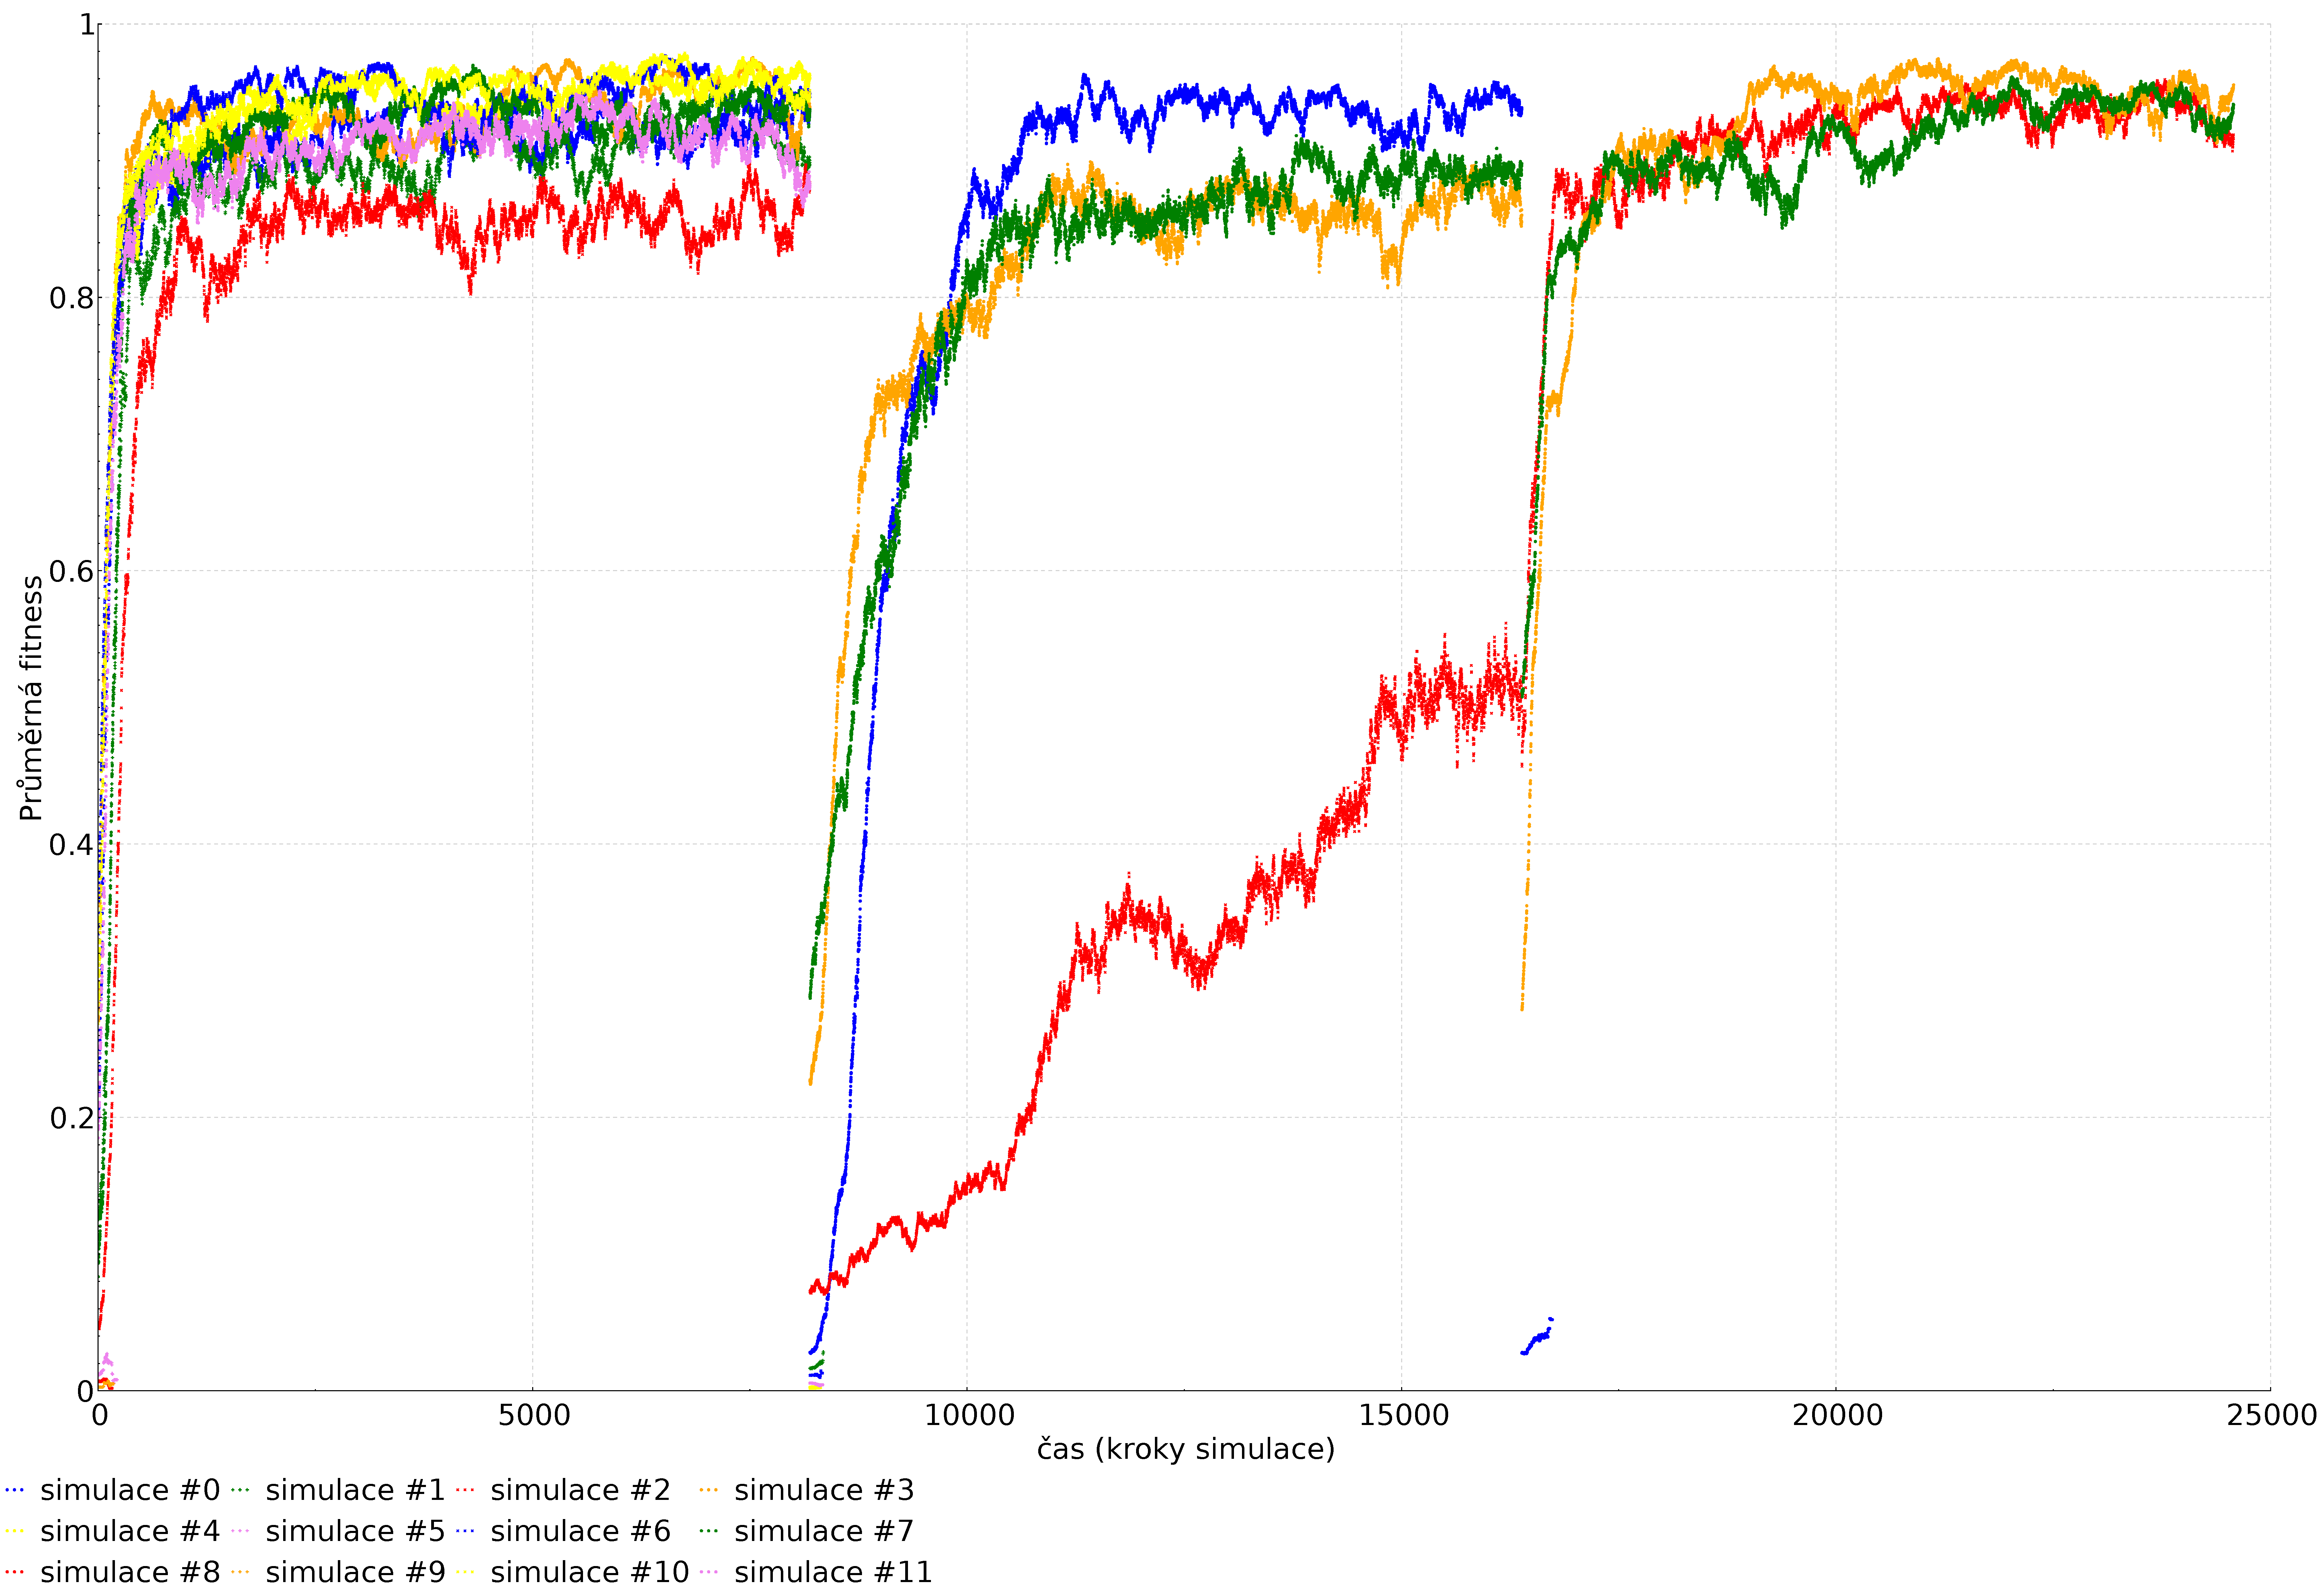
\includegraphics[width=0.8\linewidth]{img/avg_fitness_256_00_00.pdf}

\label{fig:avg_fitness_256_0.0_0.0}

\textit{Podíl alel s negativní dominancí je pravděpodobnost, že nově vzniklá alela bude ovlivňovat fenotyp v opačných
        směrech, pokud bude v lokusu jednou nebo dvakrát. Podíl pleiotropických alel je pravděpodobnost, že nově vzniklá alela
        bude ovlivňovat více složek fenotypu. Rovnovážná velikost populace byla 256 jedinců.}

\end{figure}


\begin{figure}[H]
\caption{Graf vývojů průměrně fitness dvanácti populací pro podíl vznikajících pleiotropních alel 0.25 a pro podíl
        vznikajících negativně dominantních alel 0.0}
\centering
\includegraphics[width=0.8\linewidth]{img/avg_fitness_256_25_00.pdf}

\label{fig:avg_fitness_256_0.25_0.0}

\textit{Legenda viz legenda k obrázku \ref{fig:avg_fitness_256_0.0_0.0}}

\end{figure}

\begin{figure}[H]
\caption{Graf vývojů průměrně fitness dvanácti populací pro podíl vznikajících pleiotropních alel 0.0 a pro podíl
    vznikajících negativně dominantních alel 0.5}
\centering
\includegraphics[width=0.8\linewidth]{img/avg_fitness_256_00_50.pdf}

\label{fig:avg_fitness_256_0.0_0.5}

\textit{Legenda viz legenda k obrázku \ref{fig:avg_fitness_256_0.0_0.0}}

\end{figure}

\begin{figure}[H]
\caption{Graf vývojů průměrně fitness dvanácti populací pro podíl vznikajících pleiotropních alel 0.25 a pro podíl
    vznikajících negativně dominantních alel 0.5}
\centering
\includegraphics[width=0.8\linewidth]{img/avg_fitness_256_25_50.pdf}

\label{fig:avg_fitness_256_0.25_0.5}

\textit{Legenda viz legenda k obrázku \ref{fig:avg_fitness_256_0.0_0.0}}

\end{figure}

\subsection{Desetiprocentní percentil fitness}

Stejně jako průměrná fitness roste díky selekci ve všech obdobích i desetiprocentní percentil,
přestože ne vždy stejným tempem.

\begin{figure}[H]
\caption{Graf vývojů desetiprocentního percentilu fitness dvanácti populací pro podíl vznikajících pleiotropních alel 0.0 a pro podíl
         vznikajících negativně dominantních alel 0.0}
\centering
\includegraphics[width=0.8\linewidth]{img/10percentyl_fitness_256_00_00.pdf}

\label{fig:10percentyl_fitness_256_0.0_0.0}

\textit{Legenda viz legenda k obrázku \ref{fig:avg_fitness_256_0.0_0.0}}

\end{figure}


\begin{figure}[H]
\caption{Graf vývojů desetiprocentního percentilu fitness dvanácti populací pro podíl vznikajících pleiotropních alel 0.25 a pro podíl
        vznikajících negativně dominantních alel 0.0}
\centering
\includegraphics[width=0.8\linewidth]{img/10percentyl_fitness_256_25_00.pdf}

\label{fig:10percentyl_fitness_256_0.25_0.0}

\textit{Legenda viz legenda k obrázku \ref{fig:avg_fitness_256_0.0_0.0}}

\end{figure}

\begin{figure}[H]
\caption{Graf vývojů desetiprocentního percentilu fitness dvanácti populací pro podíl vznikajících pleiotropních alel 0.0 a pro podíl
    vznikajících negativně dominantních alel 0.5}
\centering
\includegraphics[width=0.8\linewidth]{img/10percentyl_fitness_256_00_50.pdf}

\label{fig:10percentyl_fitness_256_0.0_0.5}

\textit{Legenda viz legenda k obrázku \ref{fig:avg_fitness_256_0.0_0.0}}

\end{figure}

\begin{figure}[H]
\caption{Graf vývojů desetiprocentního percentilu fitness dvanácti populací pro podíl vznikajících pleiotropních alel 0.25 a pro podíl
    vznikajících negativně dominantních alel 0.5}
\centering
\includegraphics[width=0.8\linewidth]{img/10percentyl_fitness_256_25_50.pdf}

\label{fig:10percentyl_fitness_256_0.25_0.5}

\textit{Legenda viz legenda k obrázku \ref{fig:avg_fitness_256_0.0_0.0}}

\end{figure}

\subsection{Odchylky fitness }

Směrodatné odchylky fitness často po změně vzrostou a pak v průběhu stabilních období klesají, ale není to pravidlem.

\begin{figure}[H]
\caption{Graf vývojů směrodatných odchylek fitness dvanácti populací pro podíl vznikajících pleiotropních alel 0.0 a pro podíl
         vznikajících negativně dominantních alel 0.0}
\centering
\includegraphics[width=0.8\linewidth]{img/odchylka_fitness_256_00_00.pdf}

\label{fig:odchylka_fitness_256_0.0_0.0}

\textit{Legenda viz legenda k obrázku \ref{fig:avg_fitness_256_0.0_0.0}}

\end{figure}


\begin{figure}[H]
\caption{Graf vývojů směrodatných odchylek fitness dvanácti populací pro podíl vznikajících pleiotropních alel 0.25 a pro podíl
        vznikajících negativně dominantních alel 0.0}
\centering
\includegraphics[width=0.8\linewidth]{img/odchylka_fitness_256_25_00.pdf}

\label{fig:odchylka_fitness_256_0.25_0.0}

\textit{Legenda viz legenda k obrázku \ref{fig:avg_fitness_256_0.0_0.0}}

\end{figure}

\begin{figure}[H]
\caption{Graf vývojů směrodatných odchylek fitness dvanácti populací pro podíl vznikajících pleiotropních alel 0.0 a pro podíl
    vznikajících negativně dominantních alel 0.5}
\centering
\includegraphics[width=0.8\linewidth]{img/odchylka_fitness_256_00_50.pdf}

\label{fig:odchylka_fitness_256_0.0_0.5}

\textit{Legenda viz legenda k obrázku \ref{fig:avg_fitness_256_0.0_0.0}}

\end{figure}

\begin{figure}[H]
\caption{Graf vývojů směrodatných odchylek fitness dvanácti populací pro podíl vznikajících pleiotropních alel 0.25 a pro podíl
    vznikajících negativně dominantních alel 0.5}
\centering
\includegraphics[width=0.8\linewidth]{img/odchylka_fitness_256_25_50.pdf}

\label{fig:odchylka_fitness_256_0.25_0.5}

\textit{Legenda viz legenda k obrázku \ref{fig:avg_fitness_256_0.0_0.0}}

\end{figure}


\subsection{Velikosti populací}

Velikosti populací se obvykle na počátku každého období propadnou. Dále populace buď vyhyne nebo se přizpůsobí a naroste.

\begin{figure}[H]
\caption{Graf vývojů velikosti dvanácti populací pro podíl vznikajících pleiotropních alel 0.0 a pro podíl
         vznikajících negativně dominantních alel 0.0}
\centering
\includegraphics[width=0.8\linewidth]{img/population_size_256_00_00.pdf}

\label{fig:population_size_256_0.0_0.0}

\textit{Legenda viz legenda k obrázku \ref{fig:avg_fitness_256_0.0_0.0}}

\end{figure}


\begin{figure}[H]
\caption{Graf vývojů velikosti dvanácti populací pro podíl vznikajících pleiotropních alel 0.25 a pro podíl
        vznikajících negativně dominantních alel 0.0}
\centering
\includegraphics[width=0.8\linewidth]{img/population_size_256_25_00.pdf}

\label{fig:population_size_256_0.25_0.0}

\textit{Legenda viz legenda k obrázku \ref{fig:avg_fitness_256_0.0_0.0}}

\end{figure}

\begin{figure}[H]
\caption{Graf vývojů velikosti dvanácti populací pro podíl vznikajících pleiotropních alel 0.0 a pro podíl
    vznikajících negativně dominantních alel 0.5}
\centering
\includegraphics[width=0.8\linewidth]{img/population_size_256_00_50.pdf}

\label{fig:population_size_256_0.0_0.5}

\textit{Legenda viz legenda k obrázku \ref{fig:avg_fitness_256_0.0_0.0}}

\end{figure}

\begin{figure}[H]
\caption{Graf vývojů velikosti dvanácti populací pro podíl vznikajících pleiotropních alel 0.25 a pro podíl
    vznikajících negativně dominantních alel 0.5}
\centering
\includegraphics[width=0.8\linewidth]{img/population_size_256_25_50.pdf}

\label{fig:population_size_256_0.25_0.5}

\textit{Legenda viz legenda k obrázku \ref{fig:avg_fitness_256_0.0_0.0}}

\end{figure}

\subsection{Počty unikátních alel}

Na počátku inicializace simulace vygeneruje obrovské množství unikátních alel, viz \ref{sec:individual_genes}.
Velmi rychle jejich počet radikálně klesne na biologicky smysluplné hodnoty.


\begin{figure}[H]
\caption{Graf vývojů počtu unikátních alel pro podíl vznikajících pleiotropních alel 0.0 a pro podíl
         vznikajících negativně dominantních alel 0.0}
\centering
\includegraphics[width=0.8\linewidth]{img/alelas_count_256_00_00.pdf}

\label{fig:alelas_count_256_0.0_0.0}

\textit{Legenda viz legenda k obrázku \ref{fig:avg_fitness_256_0.0_0.0}}

\end{figure}


\begin{figure}[H]
\caption{Graf vývojů počtu unikátních alel dvanácti populací pro podíl vznikajících pleiotropních alel 0.25 a pro podíl
        vznikajících negativně dominantních alel 0.0}
\centering
\includegraphics[width=0.8\linewidth]{img/alelas_count_256_25_00.pdf}

\label{fig:alelas_count_256_0.25_0.0}

\textit{Legenda viz legenda k obrázku \ref{fig:avg_fitness_256_0.0_0.0}}

\end{figure}

\begin{figure}[H]
\caption{Graf vývojů počtu unikátních alel dvanácti populací pro podíl vznikajících pleiotropních alel 0.0 a pro podíl
    vznikajících negativně dominantních alel 0.5}
\centering
\includegraphics[width=0.8\linewidth]{img/alelas_count_256_00_50.pdf}

\label{fig:alelas_count_256_0.0_0.5}

\textit{Legenda viz legenda k obrázku \ref{fig:avg_fitness_256_0.0_0.0}}

\end{figure}

\begin{figure}[H]
\caption{Graf vývojů počtu unikátních alel dvanácti populací pro podíl vznikajících pleiotropních alel 0.25 a pro podíl
    vznikajících negativně dominantních alel 0.5}
\centering
\includegraphics[width=0.8\linewidth]{img/alelas_count_256_25_50.pdf}

\label{fig:alelas_count_256_0.25_0.5}

\textit{Legenda viz legenda k obrázku \ref{fig:avg_fitness_256_0.0_0.0}}

\end{figure}
